\documentclass[10pt]{book}
\usepackage[%
	language=english,paper=a4paper,largepaper=true,%
	algorithm=false,%
	biblatexstyle=authoryear-square,
	biblatexOptions={natbib=true,backend=biber},%
	acronymOptions={smaller,printonlyused},%,withpage
]{ifiseries}
\usepackage{hyperref}
%\usepackage[language=english,theorems=numbersfirst,paper=a4paper]{ifiseries}
% <++USE language=german IF YOUR DOCUMENT WILL BE IN GERMAN ++>

% <++CHANGE PDF SETTINGS++>
\hypersetup{pdftitle=Systematic Analysis and Improvement of Edge Computing Simulators}
\hypersetup{pdfauthor=Darlin Stücker}
\hypersetup{pdfsubject=Master's Thesis}
\hypersetup{pdfkeywords=}

%\usepackage{etex}		% fix for miktex version 2.9 and above
%\reserveinserts{10}		% fix for miktex version 2.9 and above
%\usepackage{fixltx2e}	% fix for latex version from 2015 and below
%\usepackage[resetfonts]{cmap}
%\usepackage{nameref}

%\usepackage[format=hang]{caption}
%\usepackage{textcomp}
\usepackage{todonotes}

\lstset{
	frame=single,
	breaklines=true,
	numbers=left,
	numbersep=6pt,
	tabsize=3,
}

\ExecuteBibliographyOptions{sortcase=false,babel=other,backref=true,abbreviate=false}
\ExecuteBibliographyOptions{isbn=false,url=true,doi=true,eprint=false}
\addbibresource{bibliography.bib}
% <++PERHAPS CHANGE NAME OF BIBLIOGRAPHY RESOURCE ON LINE ABOVE OR ADD ADDITIONAL RESOURCES++>
\color{black}
\begin{document}

\frontmatter

\studtitlepage%
{Systematic Analysis and Improvement of Edge Computing Simulators}% title
{}% subtitle
{Darlin Stücker}% author
{Master's Thesis}% type
{\today}% date
{Software Engineering Group}% chair
{Prof. Dr. Wilhelm Hasselbring\\Hendrik Ken Reiter, M.Sc.} % advisors
\cleardoublepage
\studeidesstatt

\chapter*{Abstract}
\todo{Write this at the end}

%\section*{Acknowledgements}
%<++ACKNOWLEDGEMENTS++>

\tableofcontents
%\listoffigures
%\listoftables
\mainmatter

%% the actual thesis
%% use \include{filename} and \includeonly{filename} to organize your thesis
\chapter{Introduction}
% -----------------------------------------------------------------------------
\section{Motivation}
  With IoT devices projected to grow [\cite{7488250}, \cite{10258346}], the demand for real-time, low-latency applications has led to the development of edge computing as a complement and extension for cloud computing [\cite{ASHOURI2021100346}]
  Edge computing brings computational resources closer to data sources and end users, reducing latency, minimizing bandwidth usage and enabling applications that require immediate response times.

  However, deploying and testing edge computing solutions in real-world scenarios presents significant challenges, that consists of but not only of physical constraints like high costs, time commitments but are also very impractical for research and development purposes [\cite{ASHOURI2021100346}, \cite{7488250}].
  This has led to the development of various edge computing simulators that aim to model and simulate the behavior, performance and characteristics of distributed edge environments.
  These simulators are essential tools to analyze resource allocations, algorithms, configurations and deployment strategies before committing to a physical implementation.
  As containerized applications and orchestration platforms like Kubernetes become the standard for researchers and developers alike, the need to extend these technologies to the edge environments has become critical.


  Despite the growing number of available edge computing simulators, they all show different aspects, potentially incomplete or biased simulation environments [\cite{ASHOURI2021100346}].
  This lack of unison makes it difficult for researcher and developers to select appropriate simulation platforms and limits the development of more effective edge computing solutions.
  Particularly in the context of Kubernetes-based edge deployments, which have become increasingly prevalent, there is a gap in understanding which simulation tools best capture the complexities of container orchestration on the edge.


  Furthermore, existing simulators could focus on specific aspects of edge computing while potentially overlooking other critical factors that incluence real-world performance.
  Without a clear understanding of what constitutes a comprehensive edge computing simulator, research and development of newer simulators can become difficult and risky.

  
  The planned master's thesis therefore presents the advancing of the edge computing simulator ecoscape based on an evaluation of the edge computing simulation landscape.

% -----------------------------------------------------------------------------
\section{Document Structure}
To further explain the intention of said master's thesis, Chapter 2 introduces the main goal the master's thesis should meet.
Chapter 3 presents the necessary foundations for the presented topic, followed by the planned steps for the goal in Chapter 4.
At the end, Chapter 5 presents the currently planned schedule.
\chapter{Foundations}
This chapter establishes the theoretical, in form of conceptual foundations, as well as technical foundations, like the technical components that make up Ecoscape architecture, 
which are both essential for understanding the presented work in the subsequent chapters.

The first section introduces edge computing fundamentals, including its defining characteristics, architectural models, and the challenges that necessitate simulation-based research approaches as well as a quick glance at a few use cases and applications.
The second section explores simulation principles and methodologies, providing the theoretical framework for understanding how edge computing systems can be effectively modeled.
Subsequently, the technical foundations section examines the specific technologies employed in Ecoscape.
% ------------------------------------------
\section{Conceptual Foundations}
\subsection{Edge Computing Fundamentals}
\subsubsection{Definition and Core Characteristics}
The European Telecommunications Standards Institute (ETSI) describes edge computing as a ``system which provides an IT service environment and cloud-computing capabilities at the edge of an access network [...] in close proximity to its users'' [\cite{etsi_mec}].

Edge computing therefore represents a distributed computing paradigm that brings computation and data storage closer to the sources of data generation, fundamentally challenging the traditional centralized cloud model.
Unlike conventional cloud computing, where processing occurs in distant data centers, edge computing strategically positions computational resources at the network's periphery (also called the edge), enabling real-time data processing with minimal latency.

The core principle underlying edge computing is data locality, which represents the concept that processing data near its point of origin reduces transmission overhead and improves response times.
This approach addresses inherent limitations of cloud-centric architectures, particularly in scenarios requiring immediate decision-making or handling massive data volumes that would overwhelm network bandwidth if transmitted to centralized locations.
Edge computing environments present some distinguished key characteristics, such as:

\textbf{Ultra-low latency}: Edge nodes typically achieve response times of 1-20 milliseconds compared to cloud latencies of 100-500 milliseconds [\cite{8215403}, \cite{1019408}], making them suitable for time-critical applications such as atuonomous vehicle control or industrial automation.

\textbf{Bandwidth Optimization}: By processing data locally, edge computing reduces the volume of data transmitted across wide-area networks, which addresses the growing concern of for example network congestion in IoT-dense environments.

\textbf{Improved Reliability}: Due to being locally distributed, typical dependencies like the status of the central cloud server or a stable internet connection are no concerns in edge computing, making services more independent and more reliable.

\textbf{Enhanced Privacy and Security}: Local data processing minimizes exposure of sensitive information during transmission, addressing regulatory compliance requirements and user privacy concerns.

\subsubsection{Edge, Fog and Cloud Computing Paradigms}
The computing landscape encompasses not only edge computing but also its complementary paradigms, fog and cloud computing, that form together a continuum from centralized to distributed processing.

\textbf{Cloud computing} operates on the principle of centralized resource pooling, where vast computational resources are concentrated in geographically distributed but individually large data center.
The model excels in scenarios requiring massive computational power, extensive storage capacity and global accessibility.
However, cloud computing faces limitations in latency-sensitive applications, bandwidth-constrained environments and security-sensitive scenarios.

\textbf{Fog computing} on the other hand, is the middle ground between edge and cloud computing, by extending cloud capabilities to the network edge through a hierachical architecture.
Fog nodes serve as intermediate processing layers between end devices and cloud data centers in a region and therefore create an opportunity for regional coordination while maintaining some centralized oversight.

\begin{figure}[H]
  \centering
  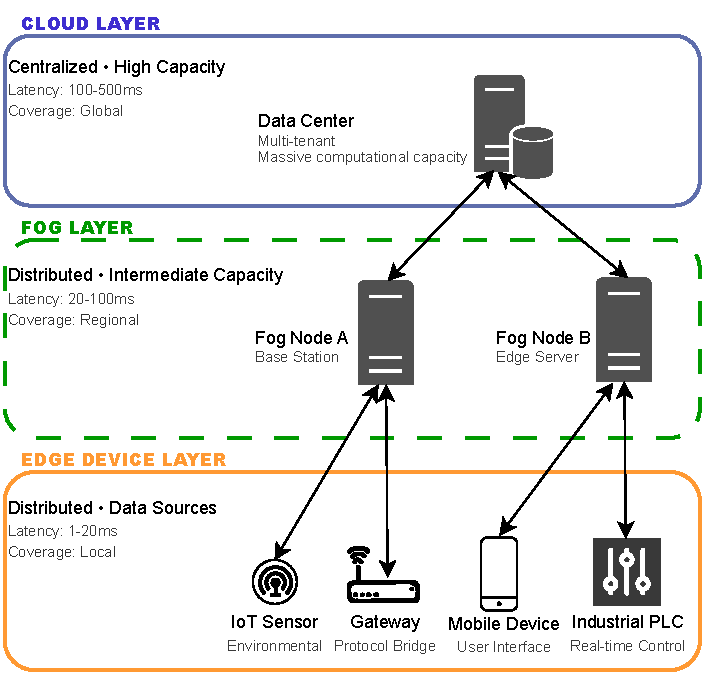
\includegraphics[width=0.75\textwidth]{img/edge_fog_cloud_diagram.pdf}
  \caption{Three-tier architecture of cloud, fog and edge computing paradigms illustrating hierachical processing distribution and data flow patterns.}
  \label{fig:edge-fog-cloud}
\end{figure}

The distinction between these paradigms often blurs in practice, as modern systems frequiently implementing hybrid approaches that leverage the strength of each layer [\cite{7488250}].
This trend can also be observed in the simulation landscape, presenting a great amount of hybrid simulators.
\subsubsection{Architectures and Deployments}
Edge computing architectures exhibit significant diversity, reflecting the varied requirements of different application domains and deployment scenarios.
However, most implementations share common structural elements that can be categorized into distinct architectural patterns.

\textbf{Three-Tier Architecture} represents the prior described, showcased in \ref{fig:edge-fog-cloud} and most prevalent design pattern, consisting of cloud, fog/edge and device layers.
In this model, lightweight edge fog nodes manage regional coordination and data aggregation, wehile cloud resources provide global oversight and resource-intensive computations.
This hierarchical approach balances computational efficiency with management complexity.

\textbf{Cloudlet-Based Architecture} focuses on the small-scale data centers positioned at network access points such as WiFi access points or cellular base stations. 
These so called cloudlets provide VM-based services to nearby mobile devices, offering a clean abstraction that simplifies application development while maintaining proximity benefits. [\cite{5280678}]

\textbf{Container-Based Edge Deployments} have gained prominence due to their lightweight nature and orchestration capabilities. Platforms like Kubernetes have been adapted for edge environments, enabling dynamic service deployment and management across heterogeneous edge infrastrcuture.
This approach aprticularly suits scenarios requiring frequent application updates or multi-tenant environments.

\textbf{Serverless Edge Computing} represents an emerging pattern where edge resources are abstracted as function-as-a-service platforms. 
This model simplifies development by allowing developers to focus on business logic rathan than infrastructure management, while the platform handles resource allocation and scaling descisions.

Deployment considerations vary significantly based on physical constraints, conncetivity patterns and operational requirements.
Industrial deployments often emphasize robustness and real-time guarantees, while mobile edge deployments prioritize energy efficiency and seamless handoff capabilities.

\subsubsection{Challenges and Requirements}
Edge computing introduces unique technical and operational challenges that distinguish it from traditional distributed systems.
These challenges stem from the fundamental trade-offs between bringing computation closer to data sources and maintaining system manageability and reliability.

\cite{7488250} describes different challenges that need to be addressed when working in this field:

\textbf{Resource Heterogeneity} describes the pool of different resource constraints regarding a wide range of diverse dvice types in edge environments. 
Unlike cloud data centers with standardized hardware configurations, edge deployments span diverse device types, from resource-constrainted IoT devices to poerful edge servers. 
This heterogeneity complicates application deployment, performance prediction and resource management strategies.

\textbf{Network Variability} in edge environments exceeds that of traditional distributed systems due to diverse connectivity options ranging from high-speed fiber connections to 
intermittent cellular or WiFi links. 
Applications must adapt to varying bandwidth, latency and reliability characteristics often requiring sophisticated fault tolerance mechanisms.

\textbf{Distributed Management Complexity} increases exponentially with the number of edge locations.
Traditional centralized management approaches become impractical when managing thousands of geographically distributed edge nodes, necessitating new approaches to monitoring, updating and maintaining edge infrastructure.

\textbf{Security and Trust} concerns are amplified in edge environments due to their geographically distribution leading to an increased attack surface and the physical accessibility of edge devices.
Edge nodes often operate in unsecured locations requiring robust security mechanisms that function independently of central authority.

\textbf{Data Consistency and Synchronization} challenges arise as the edge is a distributed system which inherits the general problem 
when multiple nodes must maintan coherent views of shared data. Additionally due to limited and intermittent connectivity to central coordination services, these challenges are further complicated and can be challenging to tackle.


\subsubsection{Use Cases and Applications}
Edge computing has found widespread adoption across diverse application domains, each presenting unique requirements that drive the evolution of edge computing architectures and technologies.
As different applications impose varying constraints on latency, reliability, processing capacity and data handling characteristics, a quick glance at the supported projects can present a valueable insight and knowledge for further discussions.

\textbf{Autonomous and Connected Vehicles} represent one of the most known and most demanding edge computing applications requiring ulta-low latency decision-making for safety-critical operations.
Edge nodes deployed at roadside infrastructure and within vehicles themselves must coordinate to procide seamless connectivity during high-speed mobility scenarios.
The computational requirements span from simple sensor data aggregation to complex computer vision and machine learning inference for object detection and path planning as well as quick decision making to guarantee the safety of everyone inside as well as outside of said vehicle. [\cite{9498627}, \cite{XIE2024}]

\textbf{Industrial Internet of Things (IIoT) and Smart Manufacturing} applications leverage edge computing to achieve real-time process control and predictive maintenance in manufacturing environments.
These deployments often require deterministic response times for safety interlocks and process control loops, demanding robust real-time operating systems and fault-tolerant architectures. [\cite{SAVAGLIO2024397}]

\textbf{Smart City Infrastructure} inherits a broad range of edge computing applications including intelligent traffic management, environmental monitoring and public safety systems.
These services extend not only to traffic but also smart waste management , air quality monitoring systems, pollution level observation and many more.
The distributed nature of smart city applications and their strong connection to IoT devices requires sophisticated coordination mechanisms to manage city-wide optimization while maintaining local autonomy for critical services. [\cite{JARARWEH2020102394}]

\textbf{Augmented and Virtual Reality (AR/VR)} applications push the boundaries of edge computing performance requirements while demanding both ultra-low latency and high computational throughput for real-time rendering and content delivery.
Mobile AR application require strong computational resources near the user to compute complex computer vision algorithms and 3D rendering. Multi-user VR environments present additional challenges by maintaining synchronized shared virtual spaces across distributed edge infrastructure. [\cite{herabad2024optimizingserviceplacementedgetocloud}, \cite{11020287}]

\textbf{Healthcare and Telemedicine} applications utilize edge computing to enable real-time patient monitoring and remote medical services while addressing strict data privacy and regulatory compliance requirements.
Wearable medical devices and IoT sensors generate continuous streams of personal medical data that must be processed locally to detect any anomalies in patients and trigger immediate alerts when necessary to guarantee the safety of the patients and detect emergencies that may go under the radar when patients are alone.
Edge-based medical analysis can provide preliminary diagnoses in remote locations where access to centralized medical expertise is limited, while ensuring that sensitive patient data remains within controlled environments. [\cite{9767142}]

These diverse application domains illustrate a few of the broad spectrum of possible projects and their respectifve requirements that edge computing system must address.
Each use case presents distinct challenges for edge computing simulators, requiring different modeling approaches for network characteristics, computational workloads, mobility patterns and failure scenarios.
Understanding the spectrum provides essential context for developing comprehensive evaluation criteria for edge computing simulation tools.

% ----------------------------------
\subsection{Simulation in Computing Systems}
\subsubsection{Principles of Discrete Event Simulation}
Discrete Event Simulation (DES) forms the theoretical foundation for most edge computing simulators, providing a mathematical framework for modeling complex distributed systems through time-ordered event processing.
Unlike continuous simulation models that evolve system state gradually over time, DES advances system state instantaneously at discrete points in time when events occur.

At its core, DES is a event-driven execution model, where system evolution is governed by a chronologically ordered sequence of events.
Each event represents a point in time when a system state change occur, such as a task arrival, task process, completion of computation or further network message delivery.
This approach particularly suits distributed computing systems, such like edge computing, as state changes are typically triggered by discrete occurrences rather than continouous processes.

For this approach, multiple mechanisms are essential for a functional DES-based simulator: [\cite{DES-sota}, \cite{DES-fptp}]

\textbf{Event Scheduling} mechanisms form the core of any DES system, as the events are the heart of the approach. The event scheduler maintains a priority quque of future events, ordered by their scheduled execution time.
When an event triggers, it may modify the system state and schedule additional future events, extending the sequence of related system behaviors.
This process terminates by either a termination condition or if the event queue becomes empty.

\textbf{State Management} in DES requires careful consideration of when and how system state change occur.
The system needs to maintain a consistent view at each simulated time point, which requires all state modifications to be atomic.
This principle becomes particularly important in distributed system simulation, where multiple concurrent events must be carefully coordinated to maintain causal relationships.

Additionally, \textbf{Random Number Generation} and \textbf{Statistical Modeling} are crucial elements for enabling stochastic behaviors inherent in real distributed systems.
Proper handling of randomness requires careful seed management for reproductibility, appropriate statistical distributiion selection for modeling system phenomena and sufficient simulation run length to achieve statiscal significance in results.

\subsubsection{Simulation vs Emulation}
For evaluating and testing edge computing tools, multiple approaches should be considered depending on the fundamental design choice that significanty impacts the capabilities, accuracy and performancy characteristics of edge computing tools.
Understanding the distinction in these approaches is crucial for both developing and selecting appropriate evaluation methodologies.

\textbf{Simulation} creates abstract models that capture the essential behavioral characteristics of target systems without implementing actual system components.
Here, scalable and controllable can be defined and typically their behavior gets modelled through statistical approximations and simplified abstractions, enabling rapid evaluation of large-scale scenarios that would be impractical to deploy in reality.
However, simulated behavior may not accurately reflect the complexity and unpredictability of real system implementations. [\cite{inproceedings-sim-vs-emu}]

\textbf{Emulation}, on the other hand, bridges the gap between simulation and real deployment by combining acutal software implementations with virtualized or abstract hardware resources.
Here, platforms execute real application code and system software while providing controlled, reproducible execution environments.
Hence, emulation typically provides higher accuracy and realistic implementation-sepcific behaviors and interactions that simulations might overlook, for the price of greater computational resources and limits that scale evaluable scenarios. [\cite{inproceedings-sim-vs-emu}]

Simulation and emulation do interrelate greatly, which results in \textbf{Hybrid} approaches being possible.
These have merged to combine the benefits of both methodologies, by using detailed emulation for critical system components while employing simulation for large-scale or less critical elements. [\cite{inproceedings-sim-vs-emu}]

The choice between simulation and emulation depends on evaluation objectives, available resources and required accuracy levels.
Development and research focusing on algorithmic performance might benefit from simulation's scalability, while studies evaluating real system deployments might require emulation's higher fidelity.

\todo{Maybe include standard performance metrics and evaluation methods ? Idk}

% ------------------------------------------
\section{Technical Foundations}
Ecoscape represents a modern approach to edge computing simulation, developed by \cite{reiter2025ecoscapefaulttolerancebenchmark} to address the growing need for realistic evaluation of containerized edge deployments.
Built upon the Kubernetes orchestration platform, Ecoscape integrates Apache Kafka for distributed data streaming, Kepler for energy consumption monitoring, Prometheus for metric collection with Grafana for visualization and Chaos Mesh for systematic reliability testing.
This creates a comprehensive simulation environment that reflexts contemporary edge computing infrastucture.

In the following, these technologies get further explored to illustrate what their direct influence is and which aspect in Ecoscapes architecture they cover.
% ----------------------------------
\subsection{Kubernetes}
Kubernetes\footnote{\url{https://kubernetes.io/}} (also known as K8s) is an open-source container orchestration platform that automates the deployment, scaling and management of containerized applications across distributed computing environments by implementing a master-worker architecture [\cite{10.5555/3175917}].
It provides a robust framework for managing microservices architectures by abstracting underlying infrastructure complexity.
Core abstractions include Pods, as the smallest deployable units, Services for network endpoints and deployments for lifecycle management.

Kubernetes has evolved from the cloud-native container orchestration platform to a fundamental standardized technology for managing distributed edge computing deployments.
Its declarative configuration model and extensive ecosystem make it particularly well-suited for the complex requirements of edge infrastucture management [\cite{10.1145/3539606}].

Edge-Specific Kubernetes Distributions suchs as K3s\footnote{\url{https://k3s.io/}} and MicroK8s\footnote{\url{https://microk8s.io/}} have merged to address the resource constraints and operational requirements of edge environments [\cite{10.1145/3578244.3583737}].
These lightweight distribution reduce memory footprint and eleminate dependencies on external databases, making them suitable for deployment on resource-constrained edge hardware while maintaining compatibility with standard Kubernetes APIs.

Furthermore, does Kubernetes support custom resource definitions (CRDs) and operators which provide mechanisms for encoding edge-specific operational knowledge into Kubernetes control plane.
Edge computing operators can therefore automate complex deployment patterns, manage application lifecycle across heterogeneous hardware and implemnt domain-specific optimization strategies while maintaining integration with standard Kubernetes tooling.

Additionally, the cluster federation and multi-cluster management capabilities of Kubernetes enable coordinated management of edge deployments across multiple geographic locations.

% ----------------------------------
\subsection{Prometheus and Grafana}
Prometheus\footnote{\url{https://prometheus.io/}} provides metrics collection and monitoring capabilities essential for observability in distributed edge computing environments.

Due to prometheus's pull-based monitoring architecture, agents to maintain persistent connections to central monitoring systems are not further required and with a time-series database, multiple metrics can be stored efficiently across a hterogeneous distributed infrastructure.
Additionally, service discovery integration allows prometheus to automatically discover and monitor new edge nodes and services as they join or leave the deployment, making it adapt to changes in a dynamic edge enviornment where node frequently change due to mobility, maintenance or scaling operations.

This all get further supported by Grafana's\footnote{\url{https://grafana.com/}} visualization capabilities which transform raw metrics data into actionable insights through customizable dashboards, alerting mechanisms and data exploration interfaces.

This seemless intergration between Prometheus and Grafana creates a complete adaptable, customizable and observable monitoring stack that enables developers and researches to understand system behavior, identify anomalies and bottlenecks as well as respond to operational issues in real-time.

% ----------------------------------
\subsection{Apache Kafka}
Apache Kafka's\footnote{\url{https://kafka.apache.org/}} (hereinafter called Kafka) distributed streaming platform capabilities address critical data management requirements in edge computing environments, particularly for scenarios requiring real-time data processing and reliable message delivery across distributed infrastructure.

The platform's partition-based scaling model allows fine-grainded control over data locality and processing distribution, which are deemed crucial capabilities for edge scenarios with bandwith constrains. With the Kafka connect ecosystem extensive integration capabilities are provided via edge data sources and sinks, which enables streamlined data pipeline construction without custom coding.
The connector framework supports various protocols, such like industrial protocols, IoT platforms and database systems, making it widely adaptable in different applications.

Sophisticated real-time analytics are enabled due to Kafka Streams processing capabilities within the Kafka ecosystem, reducing the complexity of processing architectures.
Hence, stream processing applications can implement complex event processing, data enrichment and aggregation logic while maintaining the fault tolerance and scalability charactistics of the underlying Kafka platform.
% ----------------------------------
\subsection{Kepler}
Kepler\footnote{\url{https://sustainable-computing.io/}} (Kubernetes-based Efficient Power Level Exporter) represents a specialized monitoring solution designed to provide granular energy consumption visbility in containerized edge environments.
This addresses the growing importance of energy efficiency in edge computing deployments.

The energy consumption gets calculated based on the ratio of resources used to total energy.
The total energy consumption is collected from Running Average Power Limit (RAPL) zones and other hardware sensors.
For systems the power level can be then determine by dividing the total energy into active and idle based on for example CPU usage ratio.
On the other hand, for processes the power level can be calulated by dividing the power used by a given resource based on the ratio of the process and system resource utilization.
This can not only happen with CPU usage but also for example GPU usage and other resources.

Based on that, Kepler can assign each process, system and container an energy consumption level, which becomes particularly valuable in battery-powered edge deployments where energy efficiency directly impact operational sustainability.

Additionally, Machine Learning-Based Energy Modeling capabilities enable energy consumption prediction based on workload characteristics and historical pattern. These predictive models support proactive energy management strategies and enable simulation of energy consumption under various deployment scenarios.

% ----------------------------------
\subsection{Chaos Mesh}
Chaos Mesh\footnote{\url{https://chaos-mesh.org/}} provides chaos engineering powered capabilities specifically designed for Kubernetes environments, enabling systematic reliability testing of edge computing systems under various failur conditions and operational stresses.

Under the motto of "Break Your System Constructively", Chaos Mesh allows for simulated abnormalities that might realisticly occur, such as network-level chaos experiments and resource-based chaos testing.
Here, multiple variables and failures can be simulated, including but not only network partitions, latency variations and bandwidth limitations as well as CPU throttling, memory limitations and disk space restrictions.
These experiments enable validation of application resilience to the network unreliability characteristic of edge deployments as well as evaluation at degradation behaviors and additional resource managment effictiveness.

\chapter{State-of-the-Art Simulator Analysis}
\todo{Criteria, Simulator Overview, Comparative Analysis, Highlights, Gap Analysis}
\chapter{Requirements Catalogue}
This chapter establishes a systematic requirements catalogue for edge computing simulators derived from the comparative analysis presented in the previous chapter.
The catalogue's structure is derived from the analysis framework and the requirements are categorized into mandatory criteria, which represent essential capabilities that any modern edge computing simulator must possess, and highly recommended criteria, which significantly enhance a simulator's utility but may not be essential for basic functionality.

% ----------------------------------
\section{Architectural Dimensions}
The fundamental architectural requirements define the structural foundation necessary for effective edge computing simulation.
\subsection{Mandatory Criteria}
A modular architecture represents the cornerstone requirement for modern edge computing simulators.
Modularity ensures extensibility, maintainability and the ability to adapt to evolving edge computing paradigms.
\begin{itemize}
  \item \textbf{Component-based Architecture}:
        The simulator must support clear separation of concerns between networking, computation and storage components while maintaining cohesive interaction capabilities.
  \item \textbf{Multi-Tier Support}:
        Coverage of at least two tiers of the computing continuum is essential, with simulators typically implementing either edge-fog or edge-cloud combinations.
        This minimum two-tier requirement ensures basic distributed computing scenarios can be modeled effectively.
  \item \textbf{Discrete Event Simulation (DES)}:
        The underlying simulation engine must support discrete event simulation to enable accurate temporal modeling for edge computing scenarios.
\end{itemize}

\section{Functional Capabilities}
The functional requirements define essential and desirable operational features for edge computing simulators.
\subsection{Mandatory Criteria}
Edge computing simulators must provide fundamental capabilities for modeling distributed computing environments to maintain operational effectiveness in the edge computing simulation landscape:
\begin{itemize}
  \item \textbf{Network Modeling}:
        Support for configurable network topologies, bandwidth constraints and latency modeling must be included.
        This extends to the basic routing capabilities and network protocol simulation to authentically simulate network behavior.
  \item \textbf{Device and Infrastructure Modeling}:
        Accurate representation of computational resources (CPU, memory, storage) and their constraints on heterogeneous device specifications and resource management is 
        an active criteria of edge computing simulations.
  \item \textbf{Application Workload Modeling}:
        Tasks should be schedulable and resource allocation mechanisms should be presented.
        This supports application deployment and execution modeling.
        Additionally, data generation should at least be synthetic and should follow basic data flow patterns and messaging such as streams.
  \item \textbf{Fault Tolerance Modeling}:
        Every type of simulated entity provides their own failure types that need to be detected with for example health checks and timeouts, and need to be recovered from with different strategies.
        This ensures realistic fault tolerance behavior in edge computing scenarios.
\end{itemize}

While not presented directly in the comparison but shown as significant in the gap analysis, \textbf{Energy Modeling} is positioned between mandatory and recommended requirements.
At least a basic but realistic approximation should be provided and ideally the exact energy consumption should be modeled for each device in each state.

\subsection{Recommended Criteria}
While core features are mandatory, some advanced capabilities enhance the simulator's utility significantly but are solely based on the represented focus:
\begin{itemize}
  \item \textbf{Mobility Support}:
        Device mobility modeling should influence network behavior based on realistic mobility patterns.
        This should either be achieved via synthetic or real dataset integration.
\end{itemize}

Similar to energy modeling, \textbf{Security and Privacy Modeling} is not prominently represented in the comparison.
Regardless, its importance should not be overlooked and should be considered for future research.
However, based on the abstraction to application level and the importance of mobility, it is not as highly recommended as mobility support in the current state of the edge computing simulation landscape.

% ----------------------------------
\section{Performance and Scalability}
Performance requirements ensure the simulator can handle realistic edge computing scenarios effectively.
\subsection{Mandatory Criteria}
\begin{itemize}
  \item \textbf{Basic Scalability}:
        A simulator must handle robust scenarios with a minimum of 1,000 nodes.
        Efficient resource utilization should be provided during simulation.
  \item \textbf{Execution Control}:
        Simulations are to be executed deterministically and provide reproducible results across runs.
        This needs to be managed by a scenario management system such as seed control management.
        Basic performance optimization features should be provided to ensure stable simulations.
  \item \textbf{Resource Management}:
        Memory utilization should be managed efficiently and basic parallel execution support is provided.
\end{itemize}

\subsection{Recommended Criteria}
\begin{itemize}
  \item \textbf{Advanced Scalability}:
        While basic scalability provides a foundation for edge computing simulation scenarios, large-scale scenarios are recommended.
        Distributed execution capabilities should function with scenarios of at least 10,000 nodes.
  \item \textbf{Performance Optimization}:
        To further optimize performance, multi-threading and additional memory optimization features should be provided and supported.
        Additionally, scenario acceleration capabilities are recommended.
\end{itemize}
% ----------------------------------
\section{Usability and User Experience}
Usability requirements ensure effective and user friendly utilization of the simulator.
\subsection{Mandatory Criteria}
\begin{itemize}
  \item \textbf{Documentation}:
        To ensure easy useability and further development, comprehensive setup and usage documentation is to be provided, with 2-5 basic usage examples and tutorials as well as API reference documentation.
  \item \textbf{Configuration}:
        Clear configuration mechansims should be provided to define scenarios with basic parameters.
        For this, configuration should be available as a GUI or standardized file format like YAML, INI or XML.
\end{itemize}
\subsection{Recommended Criteria}
\begin{itemize}
  \item \textbf{User Interface}:
        Idealy, the simulator has a user-friendly interface like a GUI to interact and select specific scenario parameters as well as real-time monitoring capabilities and graphical interactive visualization tools.
\end{itemize}
% ----------------------------------
\section{Validation and Evaluation}
Validation requirements ensure reliable and accurate simulation results, while also evaluating the simulator itself.
\subsection{Mandatory Criteria}
\begin{itemize}
  \item \textbf{Basic Validation}:
        Metrics must be deprived from application-level and collected on simulator-level.
        Their definition must be customizable to allow different scenarios and applications, while the export must be readable and support standardized visualization and interpretation tools like MATLAB.
        The results must be exportable in file formats like JSON or CSV.
        The format must additionally be conclusive to be validating the simulation.
  \item \textbf{Error Handling}:
        Clear error handling with comprehensive logging capabilities are essential for debugging and validation, while the system must maintain data integrity during error conditions.

\end{itemize}
\subsection{Recommended Criteria}
While not being present in most evaluated tools, in the future the catalogue can be extended by looking forward to these aspects:
\begin{itemize}
  \item \textbf{Advanced Validation}:
        Support for comparative benchmarking against other simulators or real system to ensure authentic verification of results and comparasions to other tools.
  \item \textbf{Integration Testing}:
        Integration with continous integration pipelines and validation against real-world datasets when available, can support the integration of simulated scenarios into the real-world.
\end{itemize}
% ----------------------------------
\section{Summary}
This requirements catalogue establishes clear criteria for evaluating and developing edge computing simulators.
The main aspect of a simulator is adaptability to different scenarios and evolution with the growing technology stack.
Thus, extensibility and customization in form of configuration is an aspect that is prominently considered.
Additionally, the modeling of heterogeneous devices and networks makes simulators authentic, making the requirements reflect both the current state of the art and anticipated future needs in edge computing, as identified through our comprehensive analysis.

\chapter{Ecoscape}
\todo{Description, Assessment, Gap Identification with Catalogue Enhancement Opportnunites, Agenda, Implementation}
\chapter{Evaluation}
\todo{Methodology, Description, Result}
\chapter{Conclusion and Future Work}
\todo{Write this rather at the end}

\backmatter
\tocbibliography
\end{document}
